\chapter{Conclusão}

Os acidentes de trânsito representam altos custos monetários para a sociedade. Com base na metodologia desenvolvida anteriormente pelo Ipea em conjunto com a Associação Nacional de Transportes Públicos (ANTP) e o Departamento Nacional de Trânsito (Denatran), foram atualizados os cálculos de custos dos acidentes de trânsito nas rodovias federais para a base de acidentes dos anos de 2007, 2010 e 2014.
\begin{figure}[h!]
  \centering
  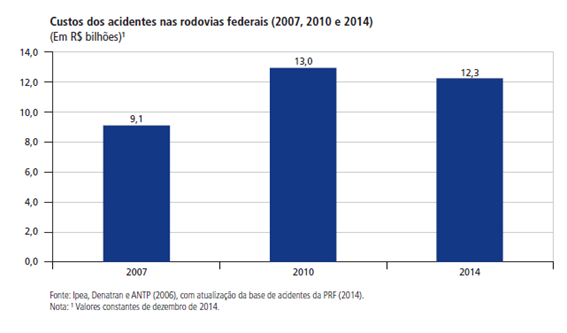
\includegraphics[width=250px, scale=1]{figuras/custos_acidentes_rodovia}
  \caption{Custos dos acidentes nas rodovias federais}
\label{fig:custos_acidentes_rodovia}
\end{figure}

Os cerca de 170 mil acidentes de trânsito ocorridos nas rodovias federais brasileiras em 2014 geraram um custo para
sociedade de R\$ 12,3 bilhões. Destes, 64,7\% estavam associados às vítimas dos acidentes, como cuidados com a saúde e
perda de produção devido às lesões ou morte, e 34,7\% aos veículos, como danos materiais e perda de cargas, além dos
procedimentos de remoção dos veículos acidentados.

Estima-se que o custo dos acidentes nas rodovias estaduais e municipais, em 2014, teria sido algo entre R\$ 24,8 e R\$ 30,5
bilhões. O estudo feito a respeito dos custos dos acidentes nas rodovias federais apontou também que acidentes com
vítimas fatais correspondem por menos de 5\% do total de ocorrências e representam cerca de 35\% dos custos totais.
Sendo que o custo médio desse tipo de acidente foi de R\$ 646.762,94. Esse dado enfatiza a necessidade de intensificar
as políticas públicas a fim de reduzir a quantidade dos acidentes e também sua gravidade \cite{ipea4}.

Neste estudo foi desenvolvido um Sistema de Comunicação Interveicular para Alerta de Colisões em Rodovias (CIAC). Com a utilização do CIAC, espera-se que o número de acidentes frontais em rodovias brasileiras diminua consideravelmente e que o sistema desenvolvido proporcione segurança para o motorista ao realizar uma ultrapassagem em trechos de pouca visibilidade, por exemplo. O dispositivo funcionará ininterruptamente, dessa forma sempre que for detectada a intenção de ultrapassagem o sistema indicará se é possível ou não seguir com a manobra. Será necessário que todos os carros próximos ao veículo com intenção de ultrapassar obtenham o sistema interveicular, somente assim, a adoção do sistema apresenta-se como uma ferramenta apta a colaborar com a diminuição de acidentes em rodovias de mão dupla.

Além disso, o CIAC deverá ser ativado ao dar partida no veículo e só poderá ser utilizado em veículos automotores, com exceção de veículos motorizados de duas ou três rodas. O seu funcionamento é baseado na comunicação interveicular composta principalmente por GPS, transponder, Lidar, Radar, sensor de rotação e câmera. Esses dispositivos foram escolhidos de forma criteriosa, conforme analisado no presente relatório, para que o sistema funcione corretamente perante algumas adversidades do clima e do relevo local.

O CIAC abrange as três engenharias. São elas a engenharia humana, a engenharia social e a engenharia física. A Engenharia Humana aborda os impactos humanos dos projetos de Engenharia e está relacionada à importância de projetar a fim de otimizar o bem-estar humano e o desempenho geral do sistema. Já a Engenharia Social lida mais com estruturas do que com funções, preocupando-se com a criação de novas formas e de novos estilos de convivência social, enquanto a Engenharia Física é relacionada ao lado mecânico e operacional do sistema.

Analisando esses 3 tipos de engenharia e tomando como base seus pesos chega-se à conclusão que o sistema deve ser implantado com base nas engenharias humana e social, pois o sistema tem o objetivo de preservar a vida. Infelizmente a engenharia física também influencia muito pois nela temos os custos envolvidos. A partir da engenharia física chega-se à conclusão que o CIAC será inviável devido aos altos custos do LIDAR e dos custos com logística e equipe para execução do projeto. Felizmente essa situação é reversível. A partir de leis que obrigam equipamentos de segurança como o Airbag e o ABS, o CIAC, em um futuro próximo também poderá ser um item obrigatório, visto sua importância social.

Dessa forma, quando a lei for implementada, os custos dos equipamentos certamente serão reduzidos (licitações serão feitas e tomadas de decisão também) visto que serão adquiridos em alta escala. Sendo assim, o principal ponto que impede a aplicação do CIAC atualmente –CUSTO- será reduzido por meio da obrigatoriedade do mesmo e sua viabilidade será alcançada a fim de cumprir com seu papel de engenharia humana e social salvando vidas.
